\documentclass[11pt, a4paper, USenglish]{article} % change ``USenglish'' to ``norsk'' if applicable.
% Search http://ctan.org or type texdoc <package name> in a terminal to access LaTeX package documentation.
\usepackage{babel} % babel and csquotes are packages for multilingual (e.g. Norwegian) support.
\usepackage[T1]{fontenc} % See http://tex.stackexchange.com/questions/664/why-should-i-use-usepackaget1fontenc
\usepackage[utf8]{inputenc} % See http://tex.stackexchange.com/questions/44694/fontenc-vs-inputenc
\usepackage{csquotes} % Needs to be loaded after inputenc.
\usepackage{amsmath} % See: http://tex.stackexchange.com/questions/32100/what-does-each-ams-package-do
\usepackage{amssymb} % See above.
\usepackage[squaren]{SIunits} % Provides SI units like \meter. The squaren option is due to a conflict with amssymb.
\usepackage{graphicx} % Provides the \includegraphics command.
\usepackage{booktabs} % Better tables. Provides \toprule, \midrule, \bottomrule.
\usepackage{listings} % Provides source code listings.
\usepackage{todonotes} % Provides several handy TODO commands.

\usepackage{biblatex} % Provides several handy TODO commands.
%\usepackage[
%  backend=bibtex,
%  style=numeric,
%  isbn=false,
%  doi=false]{biblatex} % http://tex.stackexchange.com/questions/25701/bibtex-vs-biber-and-biblatex-vs-natbib
\usepackage{hyperref} % Provides clickable links. Always load last, but before cleveref.
\usepackage{cleveref} % Provides the \Cref command, for cross-referencing of equations, sections, figures and tables. Always load last.

\addbibresource{bibliography.bib} % Makes the bibliography file available to biblatex.

% ``listings'' package settings
\definecolor{dkgreen}{rgb}{0,0.6,0}
\definecolor{gray}{rgb}{0.5,0.5,0.5}
\definecolor{pink}{rgb}{0.63, 0.13, 0.94}
\lstset{language=Matlab, 
	keywords={break, case, catch, continue,else,elseif,end,for,function,
		global,if,otherwise,persistent,return,switch,try,while},
	basicstyle=\ttfamily,
	keywordstyle=\color{blue},
	commentstyle=\color{dkgreen},
	stringstyle=\color{pink},
	numbers=left,
	numberstyle=\tiny\color{gray},
	stepnumber=1,
	numbersep=10pt,
	backgroundcolor=\color{white},
	tabsize=4,
	showspaces=false,
        showstringspaces=false}
 % The preamble specifies all included packages and related parameters.
% \input simply inserts the contents of the file, while \include forces a \newpage.
% See \input vs. \include: http://tex.stackexchange.com/questions/246/when-should-i-use-input-vs-include

\begin{document}

% Titlepage
\title{LaTeX Lab Report Template}
\author{Group 00\\Student 70000\\Student 70001\\Student 70002}
\date{January 1, 1970}
\begin{titlepage}
    \maketitle
    \begin{figure}
    \centering
    \includegraphics[width=0.5\textwidth]{figures/itk_ntnu}\\
    Department of Engineering Cybernetics
    \end{figure}
    \thispagestyle{empty}
\end{titlepage}

% Abstract
\newpage
\input{abstract}
\thispagestyle{empty} % Avoid page numbering on the abstract page.

% TOC
\newpage
\tableofcontents
\thispagestyle{empty} % Avoid page numbering on the table of contents.

% Main content
\newpage
\setcounter{page}{1}
\section{Introduction}\label{sec:intro}
Your introduction should contain an overview of the work you were assigned, as well as a few sentences putting the work into a larger perspective. You should also give a quick description of how the report is organized (as is done below).

You should of course put most of the work into doing good work in the lab and then presenting it in the report. When presenting your work in the report, both content and presentation/layout matters. Since your only way of communicating your good effort in the lab is through writing about it here, the way you write about it is essential. This means that even if you have the very best controller but describe it poorly, you will probably not be rewarded for the good results. A plot showing perfect control is worth very little if it is not accompanied by a clear description of what it represents.

Layout is naturally less important than content, but it still matters. You can think of report writing like selling an apartment; when you present your apartment for potential buyers you will of course clean the apartment and make it good looking. How clean the apartment is does of course not determine its value, but it is still important since it influences the subjective value your buyers will put on the apartment. 

\subsection{Software}
You are of course free to use whatever software you want for report writing. You can also submit a handwritten report, although this is probably not a great idea if your handwriting can be hard to read. 

You can also use Word or a similar word processor. However, it is next to impossible to achieve decent layout with Word. The support for vector graphics (discussed later) is extremely poor, and text tends to look pretty bad (bad support for kerning and ligatures). Furthermore, math is both time consuming and difficult to input, and tends to look very ugly. In general, a report written in Word looks like a draft.

It is strongly recommended to use Latex. Unless you tweak the layout too much, your report will almost certainly look very good. Although it can take a bit of effort to get started, it is also much quicker to use than Word and similar programs. The support for math and vector graphics is also great.

If you are new to Latex, you can have a look at the source for this document to get started. You can also look at the presentation by~\cite{Berland2010} (in Norwegian) or consult~\cite{Oetiker2011}. Another good reason to learn Latex is that you probably don't want to write your master's thesis in something like Word, doing so would likely be very frustrating. Being reasonably fluent in Latex before you get that far will make your thesis work much smoother.

Some of you are probably fluent in Latex and might plan to write the report using it. Please resist the temptation (if any) to change the fonts, make super fancy headers (they are not necessary for a report like this), change the margins, change the paragraph indentation and/or spacing, and similar things.

A great tool for collaborating on Latex documents is ShareLaTeX at \url{https://www.sharelatex.com/}; if you use this you won't have to install anything on your computer. Texmaker at \url{http://www.xm1math.net/texmaker/} is a good cross-platform editor. Some people like Lyx, which is a Latex editor that behaves a little bit like Word. If you prefer to compile your Latex document on the command line, the latexmk \url{https://www.ctan.org/pkg/latexmk} command is a great tool included in most TeX distributions. There is also a simple Vim plugin that uses latexmk as its backend called LaTeX-BoX \url{https://github.com/LaTeX-Box-Team/LaTeX-Box}.

\subsection{Other Comments}
Unless you have a very good reason not to, you should write the report in English. If you have problems with Latex, the solution is usually just a few Google searches away.

This report is organized as follows: \Cref{sec:prob_descr} contains some equations relevant for TTK4135, and some tips on how to create illustrations. Several \LaTeX{} tips can be foundin \Cref{sec:latex_tips}, such as how to create a table and matrix equations. \Cref{sec:figures} contains some advice on using plots from MATLAB\@. The closing remarks are in~\Cref{sec:conclusion}, respectively. \Cref{sec:matlab} contains a MATLAB file while \Cref{sec:simulink} shows an example Simulink diagram. The Bibliography can be found at the end, on page~\pageref{sec:bibliography}.

\include{part1}
\newcommand{\texMacro}[2]{\texttt{\textbackslash{#1}\{#2\}}}
\section{General LaTeX tips}\label{sec:latex_tips}
Some tips were given in \Cref{sec:intro}, and this section will elaborate with some more concrete examples.

\subsection{Matrix Equations}
Here is a matrix equation you can use as a template:
\begin{equation}
	\begin{bmatrix}
		1 &  0 &  0 & 0 & -b &  0 &  0 &  0 \\
		-a &  1 &  0 & 0 &  0 & -b &  0 &  0 \\
		0 & -a &  1 & 0 &  0 &  0 & -b &  0 \\
		0 &  0 & -a & 1 &  0 &  0 &  0 & -b                                
	\end{bmatrix}
	\begin{bmatrix} x_1 \\ x_2 \\ x_3 \\ x_4 \\ u_0 \\ u_1 \\ u_2 \\ u_3 \end{bmatrix}
	=
	\begin{bmatrix}
		ax_0 \\ 0 \\ 0 \\ 0      
	\end{bmatrix}
\end{equation}

\subsection{Tables}
If you want, you can use the source for \Cref{tab:parameters} to see how a (floating) table is made. 

Variables and symbols are always in italics, while units are not.

\begin{table}[tbp]
	\centering
	\caption{Parameters and values.}
	\begin{tabular}{llll}
		\toprule
		Symbol & Parameter & Value & Unit \\
		\midrule
		$l_a$ & Distance from elevation axis to helicopter body & $0.63$ & \meter\\
		$l_h$ & Distance from pitch axis to motor & $0.18$ & \meter\\
		$K_f$ & Force constant motor & $0.25$ & \newton\per\volt\\
		$J_e$ & Moment of inertia for elevation & $0.83$ & \kilogram\usk\meter\squared\\
		$J_t$ & Moment of inertia for travel & $0.83$ & \kilogram\usk\meter\squared\\
		$J_p$ & Moment of inertia for pitch & $0.034$ & \kilogram\usk\meter\squared\\
		$m_h$ & Mass of helicopter & $1.05$ & \kilogram\\
		$m_w$ & Balance weight & $1.87$ & \kilogram\\
		$m_g$ & Effective mass of the helicopter & $0.05$ & \kilogram\\
		$K_p$ & Force to lift the helicopter from the ground & $0.49$ & \newton\\
		\bottomrule
	\end{tabular}
\label{tab:parameters}
\end{table}

\subsection{The \texMacro{input}{} command}
By using \texMacro{input}{whatever} in your main tex file (\texttt{labreport.tex} in this case), the content of \texttt{whatever.tex} will be included in your pdf. This way you can split the contents into different files, e.g.~one for each problem of the assignment. This makes it easier to restructure the document, and arguably improves the readability of the tex files. For instance; maybe you want each problem to start on a new page? Simply add \textbackslash{newpage} before each \texMacro{input}{} command. Alternatively, you can use the \texMacro{include}{} command to achieve more or less the same effect. See~\cite{InputVsInclude} for more information.

\subsection{Citations and Reference Management}
In academic writing, it is very important to cite your sources. In Latex this is done by defining an an entry in a \emph{BibTeX} bibliography file like this (from \texttt{bibliography.bib}):
\lstinputlisting[language=Tex, firstline=1, lastline=7]{bibliography.bib}
and then using the \texttt{\textbackslash{cite}} command in your Latex document. For instance \texttt{\textbackslash{cite}\{Chen2014\}} will produce~\cite{Chen2014}.

There are many different citation styles, and a lot of customization that is possible, so please check out e.g.~\cite{BiberBibtexEtc,WikibookLatex}\footnote{Keep citation of web pages to a minimum, and consider using \url{http://web.archive.org} if you are worried that the reference may change or be removed in the future.}.

There is also a lot of useful software to manage your references. Some popular examples include JabRef (\url{http://www.jabref.org/}), Mendeley (\url{https://www.mendeley.com/}) and EndNote. JabRef is perhaps the simplest of these three, and stores all information in a \texttt{.bib} file that you can directly use in your Latex document. Both Mendeley and EndNote can export references as BibTeX.


YOLO
\include{part3}
\section{Conclusion}\label{sec:conclusion}
This does not have to be long, but try to write a few reasonable closing remarks.

\addcontentsline{toc}{section}{Appendix} % Remove this if you don't want the appendix included in the table of contents.
\appendix

\section{MATLAB Code}\label{sec:matlab}
This section should contain your MATLAB code. DO NOT attach files posted online (that you didn't write). Note that the method used to input code below does not look as pretty when the lines are too long.

\subsection{plot\_constraint.m}\label{sec:plot_constraint_m}
\lstinputlisting{code/plot_constraint.m}\section{Simulink Diagrams}\label{sec:simulink}
This section should contain your Simulink diagrams. Just like the plots, these should be in vector format, like in \Cref{fig:simulink}. Make them tidy enough to understand.

\subsection{A Simulink Diagram}
\Cref{fig:simulink} shows a Simulink diagram. You can use the \texttt{print\_simulink.m} function, included in the source code repository for this document, to export a Simulink model to EPS\@.
\begin{figure}[htb]
	\centering
		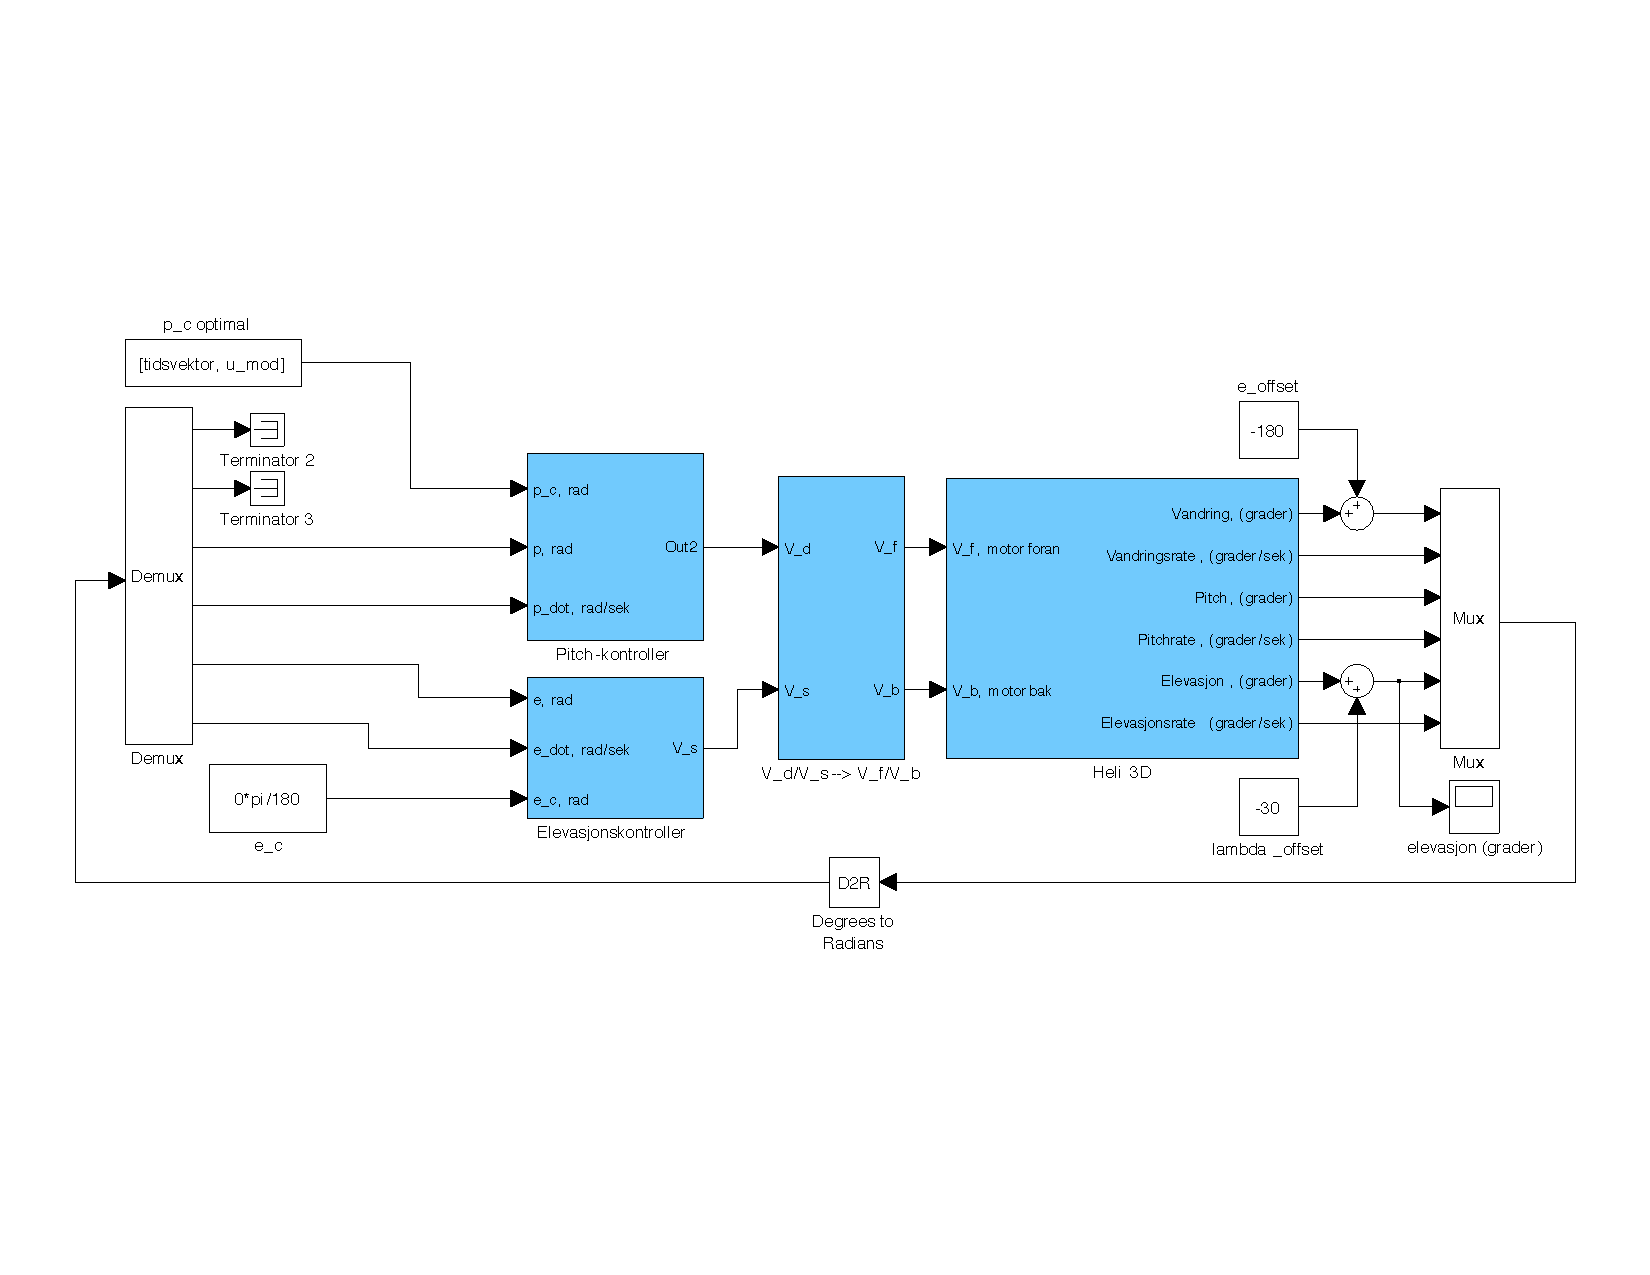
\includegraphics[width = \textwidth]{figures/simulink.pdf}
	\caption{A Simulink diagram.}
\label{fig:simulink}
\end{figure}


% References
\newpage
\addcontentsline{toc}{section}{References}
\printbibliography{}
\label{sec:bibliography}

\end{document}
